\chapter[Les boucles]{\textstyleMotCl{
Les boucles}}
{
Les ordinateurs révèlent tout leur potentiel dans leur capacité à
répéter inlassablement les mêmes tâches. Nous voyons ici comment
spécifier des boucles dans nos codes et comment les utiliser à bon
escient. \ }

\begin{center}
 [Warning: Image ignored] % Unhandled or unsupported graphics:
%\includegraphics[width=1.27cm,height=1.27cm]{log1-img/log1-img82}

\end{center}
{
Attention ! D'expérience, nous savons que ce chapitre
est difficile à appréhender par les étudiants. Beaucoup
d'entre-vous perdent pied ici. Accrochez-vous et
faites bien tous les exercices proposés !}

\begin{center}
 [Warning: Image ignored] % Unhandled or unsupported graphics:
%\includegraphics[width=1.323cm,height=1.323cm]{log1-img/log1-img83}

\end{center}
\section{La notion de travail répétitif}
{
Si on veut faire effectuer un travail répétitif, il faut indiquer deux
choses}

\liststyleNumberingi
\begin{enumerate}
\item {
Le travail à répéter}
\item {
Comment savoir s'il faut continuer la répétition ou
l'arrêter.}
\end{enumerate}
{
Examinons quelques exemples pour fixer notre propos.}

{
\textbf{Exemple 1} : Pour traiter des dossiers, on dira quelque chose
comme «~tant qu'il reste un dossier à traiter, le
traiter~» ou encore «~traiter un dossier puis passer au suivant
jusqu'à ce qu'il
n'en reste plus à traiter~».}

\liststyleListv
\begin{itemize}
\item {
La tâche à répéter est : «~traiter un dossier~»}
\item {
On indique qu'on doit continuer s'il
reste encore un dossier à traiter }
\end{itemize}
{
\textbf{Remarque :} On aurait aussi pu le formuler ainsi : «~traiter un
dossier et passer au suivant jusqu'à ce
qu'il n'en reste plus~»}

{
\textbf{Exemple 2} : Pour calculer la cote finale de tous les étudiants,
on aura quelque chose du genre «~Pour tout étudiant, calculer sa
cote~»}

\liststyleListv
\begin{itemize}
\item {
La tâche à répéter est : «~calculer la cote d'un
étudiant~»}
\item {
On indique qu'on doit le faire pour tous les étudiants.
On doit donc commencer par le premier, passer à chaque fois au suivant
et s'arrêter quand on a fini le dernier.}
\end{itemize}
{
\textbf{Exemple 3} : Pour afficher tous les nombres de 1 à 100, on aura
«~Pour tous les nombres de 1 à 100, afficher ce nombre~»}

\liststyleListv
\begin{itemize}
\item {
La tâche à répéter est : «~afficher un nombre~»}
\item {
On indique qu'on doit le faire pour tous les nombres de
1 à 100. On doit donc commencer avec 1, passer à chaque fois au nombre
suivant et s'arrêter après avoir affiché le nombre
100.}
\end{itemize}
{
\textbf{Attention} ! Comprenez bien que c'est toujours
la même tâche qui est exécutée mais pas avec le même effet à chaque
fois. Ainsi, on traite un dossier mais à chaque fois un différent; on
affiche un nombre mais à chaque fois un différent. Nous verrons comment
y arriver en logique.}

\section{Structures itératives}
{
Chacune des structures suivantes traduit une volonté de faire exécuter
un certain nombre de fois une séquence d’instructions. }

{\sffamily\bfseries
«~tant que~»}

{
Le «~tant que~» est une structure qui demande à
l'exécutant de répéter une tâche (une ou plusieurs
instructions) tant qu'une condition donnée est vraie.}

\cadre{
\begin{pseudo}
\While{condition}
	\Stmt séquence d’instructions à exécuter
\EndWhile
\end{pseudo}
}

\bigskip

{
Comme pour la structure \textstyleMotCl{si}, la \textbf{condition} est
une expression à valeur booléenne. Dans ce type de structure, il faut
qu’il y ait dans la séquence d’instructions comprise entre
\textstyleMotCl{tant que} et \textstyleMotCl{fin tant que} au moins une
instruction qui modifie une des composantes de la condition de telle
manière qu’elle puisse devenir \textbf{fausse} à un moment donné
(sinon, boucle infinie!). On fournit ci-contre un ordinogramme mettant
en évidence la dynamique de cette structure. On remarquera que si la
condition est fausse dès le début, la tâche n'est
jamais exécutée.}

{\sffamily\bfseries\upshape
«~faire – jusqu'à ce que~»}

{
Cette structure est très proche du «~tant que~» à deux différences près
:}

\liststyleNumberingi
\begin{enumerate}
\item {
Le test est fait à la fin et pas au début. La tâche est donc toujours
exécutée au moins une fois. }
\item {
On donne la condition pour arrêter et pas pour continuer; il
s'agit d'une différence mineure.}
\begin{center}
 [Warning: Image ignored] % Unhandled or unsupported graphics:
%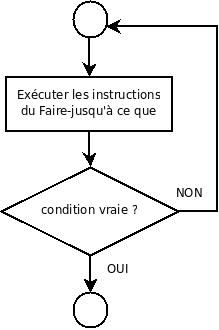
\includegraphics[width=4.302cm,height=5.313cm]{log1-img/log1-img86}

\end{center}
\end{enumerate}

\bigskip

\cadre{
\begin{pseudo}
\Repeat
	\Stmt séquence d’instructions à exécuter
\Until{condition}
\end{pseudo}
}


\bigskip

{
Comme ci-dessus, il faut que la séquence d’instructions comprise entre
\textstyleMotCl{faire} et \textstyleMotCl{jusqu'à ce
que} contienne au moins une instruction qui modifie la condition de
telle manière qu’elle puisse devenir \textbf{vraie} à un moment donné
pour arrêter l'itération. On fournit ci-contre un
ordinogramme mettant en évidence la dynamique de cette structure.}

{\sffamily\bfseries
«~pour~»}

{
Ici, on va plutôt indiquer \textbf{combien de fois} la tâche doit être
répétée. Cela se fait au travers d'une
\textbf{variable de contrôle} dont la valeur va évoluer à partir
d'une valeur de départ jusqu'à une
valeur finale.}

\cadre{
\begin{pseudo}
\For{variable \K{de} début \K{à} fin [\K{par} pas]}
	\Stmt séquence d’instructions à exécuter
\EndFor
\end{pseudo}
}

\bigskip

{
Dans ce type de structure, \textbf{début}, \textbf{fin} et \textbf{pas}
peuvent être des constantes, des variables ou des expressions (le plus
souvent à valeurs entières mais on admettra aussi des réels). Le
\textbf{pas} est facultatif, et généralement omis. Dans ce cas, la
valeur par défaut est 1. Ce pas est parfois négatif, dans le cas
d'un compte à rebours, par exemple
\textstyleCodeInsr{pour n de 10 à 1 par -1}.}

\begin{center}
 [Warning: Image ignored] % Unhandled or unsupported graphics:
%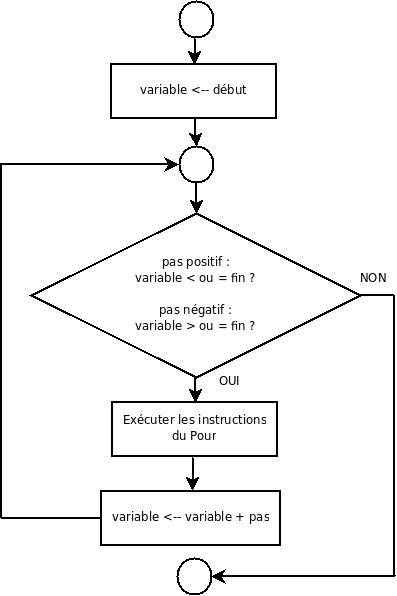
\includegraphics[width=7.004cm,height=10.516cm]{log1-img/log1-img89}

\end{center}
{
Quand le \textbf{pas} est positif, la boucle s'arrête
lorsque la variable dépasse la valeur de \textbf{fin}. Par contre, avec
un \textbf{pas} négatif, la boucle s'arrête lorsque la
variable prend une valeur plus petite que la valeur de \textbf{fin}
(cf. le test dans l'organigramme fourni)}

{
Veiller à la cohérence de l’écriture de cette structure. On considérera
qu’au cas (à éviter) où \textbf{début} est strictement supérieur à
\textbf{fin} et le \textbf{pas} est positif, la séquence d’instructions
n’est jamais exécutée (mais ce n’est pas le cas dans tous les langages
de programmation !). Idem si \textbf{début} est strictement inférieur à
\textbf{fin} mais avec un \textbf{pas} négatif.}

\begin{center}
 [Warning: Image ignored] % Unhandled or unsupported graphics:
%\includegraphics[width=1.323cm,height=1.323cm]{log1-img/log1-img90}

\end{center}
{
\textbf{Exemples~}:}

{\sffamily
\textstyleMotCl{pour} i \textstyleMotCl{de} 0 \textstyleMotCl{à} 2
\textstyleMotCl{faire} \ \ \ \ // la boucle est exécutée 3 fois}

{\sffamily
\textstyleMotCl{pour} i \textstyleMotCl{de} 2 \textstyleMotCl{à} 0
\textstyleMotCl{faire} \ \ \ \ // la boucle n'est pas
exécutée}

{\sffamily
\textstyleMotCl{pour} i \textstyleMotCl{de} 1 \textstyleMotCl{à} 10
\textstyleMotCl{par} -1 \textstyleMotCl{faire} \ \ // la boucle
n'est pas exécutée}

{\sffamily
\textstyleMotCl{pour} i \textstyleMotCl{de} 1 \textstyleMotCl{à} 1
\textstyleMotCl{par} 5 \textstyleMotCl{faire} \ \ // la boucle est
exécutée 1 fois}

{
Veiller aussi à ne pas modifier dans la séquence d’instructions une des
variables de contrôle \textbf{début}, \textbf{fin} ou \textbf{pas} ! Il
est aussi fortement déconseillé de modifier «~manuellement~» la
\textbf{variable} de contrôle au sein de la boucle
\textstyleMotCl{pour}. Il ne faut pas l’initialiser en début de boucle,
et ne pas s’occuper de sa modification, l’instruction \textbf{variable}
{\textsf{\textbf{←}}} \textbf{variable} +
\textbf{pas} étant automatique et implicite à chaque étape de la
boucle. Il est aussi déconseillé d’utiliser \textbf{variable} à la
sortie de la structure \textstyleMotCl{pour} sans lui affecter une
nouvelle valeur (son contenu pouvant varier selon le langage de
programmation).}

\begin{center}
 [Warning: Image ignored] % Unhandled or unsupported graphics:
%\includegraphics[width=1.323cm,height=1.323cm]{log1-img/log1-img91}

\end{center}
{\sffamily\bfseries
Quel type de boucle choisir ?}

{
\textstyleMotCl{\textmd{En pratique, il est possible d’utiliser
systématiquement la boucle }}\textstyleMotCl{tant
que}\textstyleMotCl{\textmd{ qui peut s’adapter dans toutes les
situations. Cependant, il est plus clair d’utiliser
}}\textstyleMotCl{pour}\textstyleMotCl{\textmd{ dans les cas où le
nombre d’itérations est fixé et connu à l’avance (par là, on veut dire
que le nombre d'itérations
}}\textstyleMotCl{\textmd{est
}}\textstyleMotCl{déterminé}\textstyleMotCl{\textmd{ au moment où on
arrive à la boucle). La boucle
}}\textstyleMotCl{faire}\textstyleMotCl{\textmd{ convient quant à elle
dans les cas où le contenu de la boucle doit être parcouru au moins une
fois, alors que dans }}\textstyleMotCl{tant
que}\textstyleMotCl{\textmd{, le nombre de parcours peut être nul si la
condition initiale est fausse. Ci-dessous un petit schéma récapitulatif
:}}}



\begin{center}
 [Warning: Image ignored] % Unhandled or unsupported graphics:
%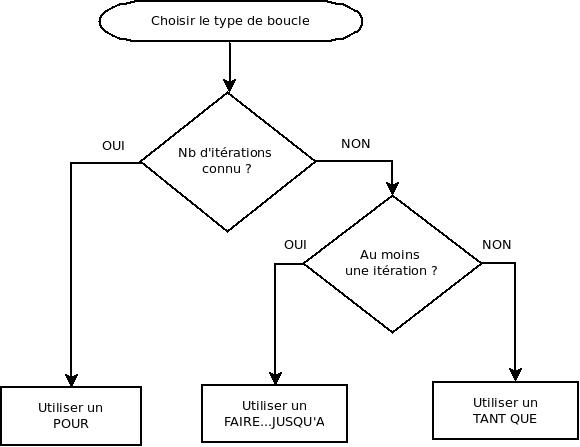
\includegraphics[width=11.044cm,height=8.509cm]{log1-img/log1-img92}

\end{center}
\section[Exemples]{\textstyleMotCl{Exemples}}
{
\textstyleMotCl{\textmd{Nous présentons quelques exemples de difficulté
croissante pour montrer comment bien utiliser les boucles.}}}

{\sffamily\bfseries\scshape
\textstyleMotCl{\textmd{Exemple 1 : Compter de 1 à 10}}}

{
\textstyleMotCl{\textmd{Imaginons qu'on veuille
afficher tous les nombres de 1 à 10. On va évidemment rejeter cette
première solution :}}}

{\sffamily
\textstyleMotCl{module}\textstyleMotCl{\textmd{ compterJusque10()}}}

{\sffamily
\textstyleMotCl{\textmd{\ \ }}\textstyleMotCl{écrire} 1}

{\sffamily
\textstyleMotCl{\textmd{\ \ }}\textstyleMotCl{écrire} 2}

{\sffamily
\textstyleMotCl{\textmd{\ \ }}\textstyleMotCl{écrire} 3}

{\sffamily
\textstyleMotCl{\textmd{\ \ }}\textstyleMotCl{écrire} 4}

{\sffamily
\textstyleMotCl{\textmd{\ \ }}\textstyleMotCl{écrire} 5}

{\sffamily
\textstyleMotCl{\textmd{\ \ }}\textstyleMotCl{écrire} 6}

{\sffamily
\textstyleMotCl{\textmd{\ \ }}\textstyleMotCl{écrire} 7}

{\sffamily
\textstyleMotCl{\textmd{\ \ }}\textstyleMotCl{écrire} 8}

{\sffamily
\textstyleMotCl{\textmd{\ \ }}\textstyleMotCl{écrire} 9}

{\sffamily
\textstyleMotCl{\textmd{\ \ }}\textstyleMotCl{écrire} 10}

{\sffamily
\textstyleMotCl{fin}\textstyleMotCl{\textmd{ }}\textstyleMotCl{module}}

{
\textstyleMotCl{\textmd{Non seulement c'est long à
écrire (imaginer l'algorithme pour afficher les
nombres de 1 à 10000 !) mais c'est très peu souple.
Cela ne fonctionne que pour 10 : il faut
}}\textstyleMotCl{\textmd{modifier l'algorithme pour
un autre décompte. La boucle va nous permettre
d'obtenir un algorithme qui s'adapte
à la limite du décompte.}}}

{
\textstyleMotCl{\textmd{Posons-nous les bonnes questions pour déterminer
la boucle :}}}

\liststyleListv
\begin{itemize}
\item {
\textstyleMotCl{\textmd{Quelle est la tâche à répéter ? Afficher un
nombre.}}}
\item {
\textstyleMotCl{\textmd{Comment savoir si on continue ? On arrête quand
«~10~» est affiché.}}}
\item {
\textstyleMotCl{\textmd{Comment afficher à chaque fois un nombre
différent ? Au travers d'une variable qui prendra
toutes les valeurs de 1 à 10. Il faut donc ajouter dans le corps de la
boucle une incrémentation de la variable}}}
\end{itemize}
{
\textstyleMotCl{\textmd{Ce qui donne :}}}

{\sffamily
\textstyleMotCl{module}\textstyleMotCl{\textmd{ compterJusque10()\ \ //
version avec tant que}}}

{\sffamily
\textstyleMotCl{\textmd{\ \ nb : entier}}}

{\sffamily
\textstyleMotCl{\textmd{\ \ nb
}}\textstyleMotCl{{←}}\textstyleMotCl{{\textmd{
1\ \ \ \ \ \ // C'est le premier nombre à
afficher}}}\textstyleMotCl{\textmd{ }}}

{\sffamily
\textstyleMotCl{\textmd{\ \ }}\textstyleMotCl{tant}\textstyleMotCl{\textmd{
}}\textstyleMotCl{que}\textstyleMotCl{\textmd{ nb
}}\textstyleMotCl{\textrm{\textmd{${\leq}$}}}\textstyleMotCl{\textmd{
10 }}\textstyleMotCl{faire}\textstyleMotCl{\textmd{\ \ // Tant que le
nb à afficher est toujours bon}}}

{\sffamily
\textstyleMotCl{\textmd{\ \ \ \ }}\textstyleMotCl{écrire}\textstyleMotCl{\textmd{
nb\ \ \ \ // On affiche la valeur de la variable nb}}}

{\sffamily
\textstyleMotCl{\textmd{\ \ \ \ nb
}}\textstyleMotCl{{←}}\textstyleMotCl{{\textmd{
nb + 1\ \ // On passe au nombre suivant}}}\textstyleMotCl{\textmd{
\ \ }}}

{\sffamily
\textstyleMotCl{\textmd{\ \ }}\textstyleMotCl{fin}\textstyleMotCl{\textmd{
}}\textstyleMotCl{tant}\textstyleMotCl{\textmd{ }}\textstyleMotCl{que}}

{\sffamily
\textstyleMotCl{fin}\textstyleMotCl{\textmd{ }}\textstyleMotCl{module}}

{
\textstyleMotCl{\textmd{Mais ici, on pourrait aussi
l'écrire avec un «~pour~» vu qu'on
connait exactement le nombre de passages dans la boucle (10). La
variable de contrôle va évoluer de 1 à 10 ce qui tombe bien car
c'est justement le nombre à afficher à chaque fois.}}}

{\sffamily
\textstyleMotCl{module}\textstyleMotCl{\textmd{ compterJusque10()\ \ //
version avec pour}}}

{\sffamily
\textstyleMotCl{\textmd{\ \ nb : entier}}}

{\sffamily
\textstyleMotCl{\textmd{\ \ }}\textstyleMotCl{pour}\textstyleMotCl{\textmd{
nb }}\textstyleMotCl{de}\textstyleMotCl{\textmd{ 1
}}\textstyleMotCl{à}\textstyleMotCl{\textmd{ 10
}}\textstyleMotCl{faire\ \ }\textstyleMotCl{\textmd{// par défaut le
pas est de 1}}}

{\sffamily
\textstyleMotCl{\textmd{\ \ \ \ }}\textstyleMotCl{écrire}\textstyleMotCl{\textmd{
nb\ \ \ \ }}}

{\sffamily
\textstyleMotCl{\textmd{\ \ }}\textstyleMotCl{fin}\textstyleMotCl{\textmd{
}}\textstyleMotCl{pour}}

{\sffamily
\textstyleMotCl{fin}\textstyleMotCl{\textmd{ }}\textstyleMotCl{module}}

{
\textstyleMotCl{\textmd{On obtient une solution plus courte et plus
lisible car l'en-tête du «~pour~» indique clairement
comment va évoluer la boucle (valeur de départ, pas et valeur
finale)}}}

{\sffamily\bfseries\scshape
\textstyleMotCl{\textmd{Exemple 2 : Compter de 1 à
}}\textstyleMotCl{\textrm{\textmd{beaucoup}}}}

{
\textstyleMotCl{\textmd{Dans l'exercice précédent, on a
affirmé que la boucle pouvait s'adapter à la limite du
décompte. Montrons-le ! Supposons qu'on veuille
afficher les nombres de 1 à n où n est une valeur donnée par
l'utilisateur.}}}

{
\textstyleMotCl{\textmd{Rien de plus simple, il suffit de lire cette
valeur au début et de l'utiliser comme limite de
boucle}}}

{\sffamily
\textstyleMotCl{module}\textstyleMotCl{\textmd{ afficherN()}}}

{\sffamily
\textstyleMotCl{\textmd{\ \ nb, n : entier}}}

{\sffamily
\textstyleMotCl{\textmd{\ \ }}\textstyleMotCl{lire}\textstyleMotCl{\textmd{
n}}}

{\sffamily
\textstyleMotCl{\textmd{\ \ }}\textstyleMotCl{pour}\textstyleMotCl{\textmd{
nb }}\textstyleMotCl{de}\textstyleMotCl{\textmd{ 1 }}\textstyleMotCl{à
}\textstyleMotCl{\textmd{n }}\textstyleMotCl{faire\ \ }}

{\sffamily
\textstyleMotCl{\textmd{\ \ \ \ }}\textstyleMotCl{écrire}\textstyleMotCl{\textmd{
nb\ \ \ \ }}}

{\sffamily
\textstyleMotCl{\textmd{\ \ }}\textstyleMotCl{fin}\textstyleMotCl{\textmd{
}}\textstyleMotCl{pour}}

{\sffamily
\textstyleMotCl{fin}\textstyleMotCl{\textmd{ }}\textstyleMotCl{module}}



\begin{center}
 [Warning: Image ignored] % Unhandled or unsupported graphics:
%\includegraphics[width=1.244cm,height=1.296cm]{log1-img/log1-img93}

\end{center}
{
\textstyleMotCl{Réflexion : }\textstyleMotCl{\textmd{Que se passe-t-il
si l'utilisateur entre une valeur négative ? }}}

{
\textstyleMotCl{\textmd{Comment améliorer le code pour que le programme
le signale à l'utilisateur ?}}}


\bigskip

{\sffamily\bfseries\scshape
\textstyleMotCl{\textmd{Exemple 3 : Afficher les nombres pairs}}}

{
\textstyleMotCl{\textmd{Cela se complique un peu. Cette fois-ci on
affiche uniquement les nombres
}}\textstyleMotCl{pairs}\textstyleMotCl{\textmd{
jusqu'à la limite n.
}}\textstyleMotCl{\textmd{Exemple}}\textstyleMotCl{\textmd{ : les
nombres pairs de 1 à 10 sont : 2, 4, 6, 8, 10}}}

{
\textstyleMotCl{\textmd{Notez que n peut être impair. Si n vaut 11,
l'affichage est le même que pour 10.}}}

{
\textstyleMotCl{\textmd{Est-ce qu'on peut utiliser un
«~pour~» ? Oui. De 1 à n, il y a exactement «~n DIV 2~» nombres à
afficher. La difficulté vient du lien à faire entre la variable de
contrôle et le nombre à afficher}}}

{
\textstyleMotCl{Solution 1}\textstyleMotCl{\textmd{ : on garde le lien
entre la variable de contrôle et le nombre à afficher. Dans ce cas, on
commence à 2 et le pas doit être de 2.}}}

{\sffamily
\textstyleMotCl{module}\textstyleMotCl{\textmd{ afficherPair()}}}

{\sffamily
\textstyleMotCl{\textmd{\ \ nb, n : entiers}}}

{\sffamily
\textstyleMotCl{\textmd{\ \ }}\textstyleMotCl{lire}\textstyleMotCl{\textmd{
n}}}

{\sffamily
\textstyleMotCl{\textmd{\ \ }}\textstyleMotCl{pour}\textstyleMotCl{\textmd{
nb }}\textstyleMotCl{de}\textstyleMotCl{\textmd{ 2
}}\textstyleMotCl{à}\textstyleMotCl{\textmd{ n
}}\textstyleMotCl{par}\textstyleMotCl{\textmd{ 2
}}\textstyleMotCl{faire\ \ }}

{\sffamily
\textstyleMotCl{\textmd{\ \ \ \ }}\textstyleMotCl{écrire}\textstyleMotCl{\textmd{
nb\ \ \ \ }}}

{\sffamily
\textstyleMotCl{\textmd{\ \ }}\textstyleMotCl{fin}\textstyleMotCl{\textmd{
}}\textstyleMotCl{pour}}

{\sffamily
\textstyleMotCl{fin}\textstyleMotCl{\textmd{ }}\textstyleMotCl{module}}

{
\textstyleMotCl{Solution 2}\textstyleMotCl{\textmd{ : la variable de
contrôle compte simplement le nombre d'itérations.
Alors il faut calculer le nombre à afficher en fonction de la variable
de contrôle (ici le double de celle-ci convient) }}}

{\sffamily
\textstyleMotCl{module}\textstyleMotCl{\textmd{ afficherPair()}}}

{\sffamily
\textstyleMotCl{\textmd{\ \ i, n : entiers}}}

{\sffamily
\textstyleMotCl{\textmd{\ \ }}\textstyleMotCl{lire}\textstyleMotCl{\textmd{
n}}}

{\sffamily
\textstyleMotCl{\textmd{\ \ }}\textstyleMotCl{pour}\textstyleMotCl{\textmd{
i }}\textstyleMotCl{de}\textstyleMotCl{\textmd{ 1
}}\textstyleMotCl{à}\textstyleMotCl{\textmd{ n
}}\textstyleMotCl{\textmd{DIV}}\textstyleMotCl{\textmd{ 2
}}\textstyleMotCl{faire}}

{\sffamily
\textstyleMotCl{\textmd{\ \ \ \ }}\textstyleMotCl{écrire}\textstyleMotCl{\textmd{
2 * i\ \ \ \ }}}

{\sffamily
\textstyleMotCl{\textmd{\ \ }}\textstyleMotCl{fin}\textstyleMotCl{\textmd{
}}\textstyleMotCl{pour}}

{\sffamily
\textstyleMotCl{fin}\textstyleMotCl{\textmd{ }}\textstyleMotCl{module}}

{
\textstyleMotCl{\textmd{Par une vieille habitude des
programmeurs}}\footnote{Née avec le langage FORTRAN où la variable
«~i~» était par défaut une variable entière.}\textstyleMotCl{\textmd{,
une variable de contrôle qui se contente de compter les passages dans
la boucle est souvent nommée «~i~». On l'appelle aussi
«~itérateur~».}}}

{\sffamily\bfseries\scshape
\textstyleMotCl{\textmd{Exemple 4 : Afficher les premiers nombres
pairs}}}

{
\textstyleMotCl{\textmd{Voici un problème proche du précédent : on
affiche cette fois les N premiers nombres pairs.
}}\textstyleMotCl{\textmd{Exemple}}\textstyleMotCl{\textmd{ : les 10
premiers nombres pairs sont : 2, 4, 6, 8, 10, 12, 14, 16, 18, 20.}}}

{
\textstyleMotCl{\textmd{Il est plus simple de partir de la solution 2 de
l'exemple précédent en changeant simplement la valeur
finale de la boucle. }}}

{\sffamily
\textstyleMotCl{module}\textstyleMotCl{\textmd{ afficherPair()}}}

{\sffamily
\textstyleMotCl{\textmd{\ \ i, n : entier}}}

{\sffamily
\textstyleMotCl{\textmd{\ \ }}\textstyleMotCl{lire}\textstyleMotCl{\textmd{
n}}}

{\sffamily
\textstyleMotCl{\textmd{\ \ }}\textstyleMotCl{pour}\textstyleMotCl{\textmd{
i }}\textstyleMotCl{de}\textstyleMotCl{\textmd{ 1
}}\textstyleMotCl{à}\textstyleMotCl{\textmd{ n
}}\textstyleMotCl{faire}}

{\sffamily
\textstyleMotCl{\textmd{\ \ \ \ }}\textstyleMotCl{écrire}\textstyleMotCl{\textmd{
2 * i\ \ \ \ }}}

{\sffamily
\textstyleMotCl{\textmd{\ \ }}\textstyleMotCl{fin}\textstyleMotCl{\textmd{
}}\textstyleMotCl{pour}}

{\sffamily
\textstyleMotCl{fin}\textstyleMotCl{\textmd{ }}\textstyleMotCl{module}}

{\sffamily\bfseries\scshape
\textstyleMotCl{\textmd{Exemple 5 : Somme de nombres}}}

{
\textstyleMotCl{\textmd{Changeons de problème. On veut pouvoir calculer
la somme d'une série de nombres donnés par
l'utilisateur. Il faut d'abord se
demander comment l'utilisateur va pouvoir indiquer
combien de nombres il faut additionner ou quand est-ce que le dernier
nombre à additionner a été entré. Voyons quelques possibilités.}}}

{
\textstyleMotCl{Variante 1}\textstyleMotCl{ :}\textstyleMotCl{\textmd{
\ L'utilisateur indique le nombre de termes au départ.
Ce problème est proche de ce qui a déjà été fait.}}}

{\sffamily
\textstyleMotCl{module}\textstyleMotCl{\textmd{ sommeNombres()\ \ \ \ //
variante 1\ \ }}}

{\sffamily
\textstyleMotCl{\textmd{\ \ nbValeurs : entier\ \ // nb de valeurs à
additionner}}}

{\sffamily
\textstyleMotCl{\textmd{\ \ valeur : entier\ \ \ \ // un des termes de
l'addition}}}

{\sffamily
\textstyleMotCl{\textmd{\ \ somme : entier\ \ \ \ // la somme}}}

{\sffamily
\textstyleMotCl{\textmd{\ \ i : entier\ \ \ \ \ \ // itérateur}}}


\bigskip

{\sffamily
\textstyleMotCl{\textmd{\ \ somme
}}\textstyleMotCl{{←}}\textstyleMotCl{{\textmd{
0\ \ \ \ // la somme se construit petit à petit. 0 au
départ}}}\textstyleMotCl{\textmd{ }}}

{\sffamily
\textstyleMotCl{\textmd{\ \ }}\textstyleMotCl{lire}\textstyleMotCl{\textmd{
nbValeurs}}}

{\sffamily
\textstyleMotCl{\textmd{\ \ }}\textstyleMotCl{pour}\textstyleMotCl{\textmd{
i }}\textstyleMotCl{de}\textstyleMotCl{\textmd{ 1
}}\textstyleMotCl{à}\textstyleMotCl{\textmd{ nbValeurs
}}\textstyleMotCl{faire}}

{\sffamily
\textstyleMotCl{\textmd{\ \ \ \ }}\textstyleMotCl{lire}\textstyleMotCl{\textmd{
valeur}}}

{\sffamily
\textstyleMotCl{\textmd{\ \ \ \ somme
}}\textstyleMotCl{{←}}\textstyleMotCl{{\textmd{
somme + valeur}}}}

{\sffamily
\textstyleMotCl{\textmd{\ \ }}\textstyleMotCl{fin}\textstyleMotCl{\textmd{
}}\textstyleMotCl{pour}}

{\sffamily
\textstyleMotCl{\ \ }\textstyleMotCl{écrire} somme}

{\sffamily
\textstyleMotCl{fin}\textstyleMotCl{\textmd{ }}\textstyleMotCl{module}}

{
\textstyleMotCl{Variante 2}\textstyleMotCl{\textmd{ : Après chaque
nombre, on demande à l'utilisateur
s'il y a encore un nombre à \ additionner. }}}

{
\textstyleMotCl{\textmd{Ici, il faut chercher une solution différente
car on ne connait pas au départ le nombre de valeurs à additionner et
donc le nombre de passages dans la boucle. On va devoir passer à un
«~tant que~» ou un «faire jusqu'à ce que». On peut
envisager de demander en fin de boucle s'il reste
encore un nombre à additionner. Ce qui donne :}}}

{\sffamily
\textstyleMotCl{module}\textstyleMotCl{\textmd{ sommeNombres()\ \ \ \ //
variante 2a\ \ }}}

{\sffamily
\textstyleMotCl{\textmd{\ \ encore : booléen\ \ // est-ce
qu'il reste encore une valeur à additionner ?}}}

{\sffamily
\textstyleMotCl{\textmd{\ \ valeur : entier\ \ \ \ // une des valeurs à
additionner}}}

{\sffamily
\textstyleMotCl{\textmd{\ \ somme : entier\ \ \ \ // la somme}}}


\bigskip

{\sffamily
\textstyleMotCl{\textmd{\ \ somme
}}\textstyleMotCl{{←}}\textstyleMotCl{{\textmd{
0\ \ \ \ // la somme se construit petit à petit. 0 au
départ}}}\textstyleMotCl{\textmd{ }}}

{\sffamily
\textstyleMotCl{\textmd{\ \ }}\textstyleMotCl{faire}}

{\sffamily
\textstyleMotCl{\textmd{\ \ \ \ }}\textstyleMotCl{lire}\textstyleMotCl{\textmd{
valeur}}}

{\sffamily
\textstyleMotCl{\textmd{\ \ \ \ somme
}}\textstyleMotCl{{←}}\textstyleMotCl{{\textmd{
somme + valeur}}}}

{\sffamily
\textstyleMotCl{{\textmd{\ \ \ \ }}}\textstyleMotCl{{lire}}\textstyleMotCl{{\textmd{
encore}}}}

{\sffamily
\textstyleMotCl{\textmd{\ \ }}\textstyleMotCl{jusqu'à
ce que }NON encore}

{\sffamily
\textstyleMotCl{\ \ }\textstyleMotCl{écrire} somme}

{\sffamily
\textstyleMotCl{fin}\textstyleMotCl{\textmd{ }}\textstyleMotCl{module}}

{
\textstyleMotCl{\textmd{Avec cette solution, on additionne au moins une
valeur. Si on veut pouvoir tenir }}\textstyleMotCl{\textmd{compte du
cas très particulier où l'utilisateur ne veut
additionner aucune valeur, il faut utiliser un «~tant que~» et donc
poser la question avant d'entrer dans la boucle.}}}

{\sffamily
\textstyleMotCl{module}\textstyleMotCl{\textmd{ sommeNombres()\ \ \ \ //
variante 2b\ \ }}}

{\sffamily
\textstyleMotCl{\textmd{\ \ encore : booléen\ \ // est-ce
qu'il reste encore une valeur à additionner ?}}}

{\sffamily
\textstyleMotCl{\textmd{\ \ valeur : entier\ \ \ \ // une des valeurs à
\ additionner}}}

{\sffamily
\textstyleMotCl{\textmd{\ \ somme : entier\ \ \ \ // la somme}}}


\bigskip

{\sffamily
\textstyleMotCl{\textmd{\ \ somme
}}\textstyleMotCl{{←}}\textstyleMotCl{{\textmd{
0\ \ \ \ // la somme se construit petit à petit. 0 au
départ}}}\textstyleMotCl{\textmd{ }}}

{\sffamily
\textstyleMotCl{{\textmd{\ \ }}}\textstyleMotCl{{lire}}\textstyleMotCl{{\textmd{
encore}}}}

{\sffamily
\textstyleMotCl{\textmd{\ \ }}\textstyleMotCl{tant que }encore
\textstyleMotCl{faire}}

{\sffamily
\textstyleMotCl{\textmd{\ \ \ \ }}\textstyleMotCl{lire}\textstyleMotCl{\textmd{
valeur}}}

{\sffamily
\textstyleMotCl{\textmd{\ \ \ \ somme
}}\textstyleMotCl{{←}}\textstyleMotCl{{\textmd{
somme + valeur}}}}

{\sffamily
\textstyleMotCl{{\textmd{\ \ \ \ }}}\textstyleMotCl{{lire}}\textstyleMotCl{{\textmd{
encore}}}}

{\sffamily
\textstyleMotCl{\textmd{\ \ }}\textstyleMotCl{fin}\textstyleMotCl{\textmd{
}}\textstyleMotCl{tant}\textstyleMotCl{\textmd{ }}\textstyleMotCl{que}}

{\sffamily
\textstyleMotCl{\ \ }\textstyleMotCl{écrire} somme}

{\sffamily
\textstyleMotCl{fin}\textstyleMotCl{\textmd{ }}\textstyleMotCl{module}}

{
\textstyleMotCl{Variante 3}\textstyleMotCl{\textmd{ :
L'utilisateur entre une valeur spéciale pour indiquer
la fin. On parle de valeur
}}\textstyleMotCl{sentinelle}\textstyleMotCl{\textmd{. Ceci
n'est possible que si cette valeur
}}\textstyleMotCl{sentinelle}\textstyleMotCl{\textmd{ ne peut pas être
un terme valide de l'addition. Par exemple, si on veut
additionner des nombres positifs uniquement, la valeur -1 peut servir
de valeur sentinelle. Mais sans limite sur les nombres à additionner
(positifs, négatifs ou nuls) il n'est pas possible de
choisir une sentinelle.}}}

{
\textstyleMotCl{\textmd{Ici, on se base sur la valeur entrée pour
décider si on continue ou pas. Il faut donc
}}\textstyleMotCl{toujours}\textstyleMotCl{\textmd{ effectuer un test
après une lecture de valeur. C'est pour cela
qu'il faut effectuer une lecture avant et une autre à
la fin de la boucle.}}}

{\sffamily
\textstyleMotCl{module}\textstyleMotCl{\textmd{ sommeNombres()\ \ \ \ //
variante 3\ \ }}}

{\sffamily
\textstyleMotCl{\textmd{\ \ valeur : entier\ \ \ \ // une des valeurs à
additionner}}}

{\sffamily
\textstyleMotCl{\textmd{\ \ somme : entier\ \ \ \ // la somme}}}


\bigskip

{\sffamily
\textstyleMotCl{\textmd{\ \ somme
}}\textstyleMotCl{{←}}\textstyleMotCl{{\textmd{
0\ \ \ \ // la somme se construit petit à petit. 0 au
départ}}}\textstyleMotCl{\textmd{ }}}

{\sffamily
\textstyleMotCl{{\textmd{\ \ }}}\textstyleMotCl{{lire}}\textstyleMotCl{{\textmd{
valeur}}}}

{\sffamily
\textstyleMotCl{\textmd{\ \ }}\textstyleMotCl{tant que} valeur ${\neq}$
-1 \textstyleMotCl{faire}}

{\sffamily
\textstyleMotCl{\textmd{\ \ \ \ somme
}}\textstyleMotCl{{←}}\textstyleMotCl{{\textmd{
somme + valeur}}}}

{\sffamily
\textstyleMotCl{\textmd{\ \ \ \ }}\textstyleMotCl{lire}\textstyleMotCl{\textmd{
valeur\ \ \ \ // remarquer l'endroit où on lit une
valeur.}}}

{\sffamily
\textstyleMotCl{\textmd{\ \ }}\textstyleMotCl{fin}\textstyleMotCl{\textmd{
}}\textstyleMotCl{tant}\textstyleMotCl{\textmd{ }}\textstyleMotCl{que}}

{\sffamily
\textstyleMotCl{\ \ }\textstyleMotCl{écrire} somme}

{\sffamily
\textstyleMotCl{fin}\textstyleMotCl{\textmd{ }}\textstyleMotCl{module}}

{
\textstyleMotCl{\textmd{Voilà ! Vous devriez à présent être en mesure de
résoudre les exercices qui suivent. Courage ! Et n'en
passez aucun !}}}

{
\textstyleMotCl{Réflexion}\textstyleMotCl{\textmd{ : Quelle valeur
sentinelle prendrait-on pour additionner une série de cotes
d'interrogations ? Une série de températures ? }}}

\begin{center}
 [Warning: Image ignored] % Unhandled or unsupported graphics:
%
\includegraphics[width=1.244cm,height=1.296cm]{log1-img/log1-img94}

\end{center}
{
\textstyleMotCl{Réflexion}\textstyleMotCl{\textmd{ : Dans les solutions
2 et 3 on lit une variable booléenne. Comment un programmeur
pourrait-il réaliser cette instruction de façon pratique ?}}}


\bigskip


\bigskip


\bigskip


\bigskip

\section[Exercices]{\textstyleMotCl{Exercices}}
\liststyleExercice
\begin{enumerate}
\item {\sffamily\bfseries
Compréhension d'algorithmes}
\end{enumerate}
{
Quels sont les affichages réalisés lors de l'exécution
des algorithmes suivants ?}

{\sffamily
\textstyleMotCl{module} boucle1\textstyleMotCl{\textmd{()}}}

{\sffamily
\ \ x : entier}

{\sffamily
\texttt{\ \ }x\texttt{
}\textstyleMotCl{{←}}\texttt{ }0}

{\sffamily
\ \ \textstyleMotCl{tant que} x {\textless} 12 \textstyleMotCl{faire}}

{\sffamily
\texttt{\ \ \ \ }x\texttt{
}\textstyleMotCl{{←}}\texttt{ }x + 2}

{\sffamily
\ \ \textstyleMotCl{fin tant que}}

{\sffamily
\ \ \textstyleMotCl{{écrire}} x}

{\sffamily
\textstyleMotCl{fin} \textstyleMotCl{module}}


\bigskip

{\sffamily
\textstyleMotCl{module} boucle2()}

{\sffamily
\ \ ok : booléen}

{\sffamily
\ \ x : entier}

{\sffamily
\ \ ok \textstyleMotCl{{←}} vrai}

{\sffamily
\ \ x \textstyleMotCl{{←}} 5}

{\sffamily
\ \ \textstyleMotCl{tant que} ok \textstyleMotCl{faire}}

{\sffamily
{\ \ \ \ x
}\textstyleMotCl{{←}}{ x
+ 7}}

{\sffamily
{\ \ \ \ ok
}\textstyleMotCl{{←}}{ x
MOD 11 }{${\neq}$}{ 0}}

{\sffamily
\ \ \textstyleMotCl{fin tant que}}

{\sffamily
\ \ \textstyleMotCl{{écrire}} x}

{\sffamily
\textstyleMotCl{fin} \textstyleMotCl{module}}


\bigskip

{\sffamily
\textstyleMotCl{module} boucle3()}

{\sffamily
\ \ ok : booléen}

{\sffamily
\ \ cpt, x : entiers}

{\sffamily
\texttt{\ \ }x\texttt{
}\textstyleMotCl{{←}}\texttt{ }10}

{\sffamily
\texttt{\ \ }cpt\texttt{
}\textstyleMotCl{{←}}\texttt{ }0}

{\sffamily
\texttt{\ \ }ok\texttt{
}\textstyleMotCl{{←}}\texttt{ }vrai}

{\sffamily
\ \ \textstyleMotCl{tant que} ok ET cpt {\textless} 3
\textstyleMotCl{faire}}

{\sffamily
\ \ \ \ \textstyleMotCl{si} x MOD 2 = 0 \textstyleMotCl{alors}}

{\sffamily
{\texttt{\ \ \ \ \ \ }}{x}{\texttt{
}}\textstyleMotCl{{←}}{\texttt{
}}{x + 1}}

{\sffamily
{\texttt{\ \ \ \ \ \ }}{ok}{\texttt{
}}\textstyleMotCl{{←}}{\texttt{
}}{x {\textless} 20}}

{\sffamily
\ \ \ \ \textstyleMotCl{{sinon}}}

{\sffamily
{\texttt{\ \ \ \ \ \ }}{x}{\texttt{
}}\textstyleMotCl{{←}}{\texttt{
}}{x + 3}}

{\sffamily
{\texttt{\ \ \ \ \ \ }}{cpt}{\texttt{
}}\textstyleMotCl{{←}}{\texttt{
}}{cpt + 1}}

{\sffamily
\ \ \ \ \textstyleMotCl{fin si}}

{\sffamily
\ \ \ \ \textstyleMotCl{{écrire}} x}

{\sffamily
\ \ \textstyleMotCl{fin tant que}}

{\sffamily
\ \ \textstyleMotCl{{écrire}} cpt}

{\sffamily
\textstyleMotCl{fin} \textstyleMotCl{module}}


\bigskip

{\sffamily
\textstyleMotCl{module} boucle4()}

{\sffamily
\ \ pair, grand : booléens}

{\sffamily
\ \ p, x : entiers}

{\sffamily
\texttt{\ \ }x\texttt{
}\textstyleMotCl{{←}}\texttt{ }1}

{\sffamily
\texttt{\ \ }p\texttt{
}\textstyleMotCl{{←}}\texttt{ }1}

{\sffamily
\ \ \textstyleMotCl{faire}}

{\sffamily
\texttt{\ \ \ \ }p \textstyleMotCl{{←}} 2 * p}

{\sffamily
\ \ \ \ x \textstyleMotCl{{←}} x + p}

{\sffamily
\ \ \ \ pair \textstyleMotCl{{←}} x MOD 2 = 0}

{\sffamily
\ \ \ \ grand \textstyleMotCl{{←}} x
{\textgreater} 15}

{\sffamily
\ \ \textstyleMotCl{jusqu'à ce que} pair OU grand}

{\sffamily
\ \ \textstyleMotCl{{écrire}} x}

{\sffamily
\textstyleMotCl{fin} \textstyleMotCl{module}}


\bigskip

{\sffamily
\textstyleMotCl{module} boucle5()}

{\sffamily
\ \ i, x : entiers}

{\sffamily
\ \ ok : booléen}

{\sffamily
\texttt{\ \ }x \textstyleMotCl{{←}} 3}

{\sffamily
\ \ ok \textstyleMotCl{{←}} vrai}

{\sffamily
\ \ \textstyleMotCl{pour} i de 1 \textstyleMotCl{à} 5
\textstyleMotCl{faire}}

{\sffamily
{\texttt{\ \ }}{\ \ x
}\textstyleMotCl{{←}}{
x + i}}

{\sffamily
{\ \ \ \ ok
}\textstyleMotCl{{←}}{
ok }{ET}{ (x
}{MOD}{ 2 = 0)}}

{\sffamily
\ \ \textstyleMotCl{fin pour}}

{\sffamily
\ \ \textstyleMotCl{si} ok \textstyleMotCl{alors}}

{\sffamily
\ \ \ \ \textstyleMotCl{{écrire}} x}

{\sffamily
\ \ \textstyleMotCl{{sinon}}}

{\sffamily
\ \ \ \ \textstyleMotCl{{écrire}} 2 * x}

{\sffamily
\ \ \textstyleMotCl{fin si}}

{\sffamily
\textstyleMotCl{fin} \textstyleMotCl{module}}


\bigskip

{\sffamily
\textstyleMotCl{module} boucle6()}

{\sffamily
\ \ i, j, fin : entiers}

{\sffamily
\ \ \textstyleMotCl{pour} i de 1 à 3 \textstyleMotCl{faire}}

{\sffamily
\ \ \ \ fin \textstyleMotCl{{←}} 6 * i - 11}

{\sffamily
\ \ \ \ \textstyleMotCl{pour} j de 1 à fin \textstyleMotCl{par} 3
\textstyleMotCl{faire} }

{\sffamily
\ \ \ \ \ \ \textstyleMotCl{{écrire}} 10 * i +
j}

{\sffamily
{\ \ \ \ }\textstyleMotCl{{fin
pour}} \ \ \ \ \ }

{\sffamily
\ \ \textstyleMotCl{fin pour}}

{\sffamily
\textstyleMotCl{fin module}}


\bigskip

\liststyleExercice
\setcounter{saveenum}{\value{enumi}}
\begin{enumerate}
\setcounter{enumi}{\value{saveenum}}
\item {\sffamily\bfseries
Simplification}
\end{enumerate}
{
Voici quelques extraits d’algorithmes corrects du point de vue de la
syntaxe mais contenant des lignes inutiles ou des lourdeurs d’écriture.
Remplacer ces portions d’algorithme par un minimum d’instructions qui
auront un effet équivalent.}

{\sffamily
a \textstyleMotCl{{←}} 1}

{\sffamily
b \textstyleMotCl{{←}} 1}

{\sffamily
\textstyleMotCl{tant que} a {\textless} 10 \textstyleMotCl{faire}}

{\sffamily
\ \ {a
}\textstyleMotCl{{←}}{
a + 1}}

{\sffamily
{\ \ b
}\textstyleMotCl{{←}}{
b + 1}}

{\sffamily
{\ \ }\textstyleMotCl{{écrire}}{
b}}

{\sffamily
\textstyleMotCl{fin tant que}}


\bigskip

{\sffamily
a \textstyleMotCl{{←}} 1}

{\sffamily
b \textstyleMotCl{{←}} 1}

{\sffamily
\textstyleMotCl{tant que} a {\textless} 10 \textstyleMotCl{faire}}

{\sffamily
\ \ {a
}\textstyleMotCl{{←}}{
a + 1}}

{\sffamily
{\ \ b
}\textstyleMotCl{{←}}{
b + 1}}

{\sffamily
\textstyleMotCl{fin tant que}}

{\sffamily
\textstyleMotCl{{écrire}}{
b}}


\bigskip

{\sffamily
i \textstyleMotCl{{←}} 1}

{\sffamily
\textstyleMotCl{pour} i de 1 à 10 \textstyleMotCl{faire}}

{\sffamily
{\texttt{\ \ }}{b}{\texttt{
}}\textstyleMotCl{{←}}{\texttt{
}}{i}}

{\sffamily
\textstyleMotCl{fin pour}}


\bigskip

\liststyleExercice
\setcounter{saveenum}{\value{enumi}}
\begin{enumerate}
\setcounter{enumi}{\value{saveenum}}
\item {\sffamily\bfseries
Afficher les n premiers}
\end{enumerate}
{
Écrire un algorithme qui lit un naturel n et affiche}

\begin{itemize}
\item {
les n premiers entiers strictement positifs ;}
\item {
les n premiers entiers strictement positifs en ordre décroissant ;}
\item {
les n premiers carrés parfaits ;}
\item {
les n premiers naturels impairs ;}
\item {
les naturels impairs qui sont inférieurs ou égaux à n.}
\end{itemize}
\liststyleExercice
\begin{enumerate}
\item {\sffamily\bfseries
Maximum de nombres}
\end{enumerate}
{
Écrire un algorithme qui lit une série de cotes d’interrogation (entiers
entre 0 et 20) et affiche ensuite la plus grande. Pour signaler la fin
de l’encodage des cotes, l’utilisateur introduit un nombre négatif
(\textbf{valeur sentinelle}).}

\liststyleExercice
\setcounter{saveenum}{\value{enumi}}
\begin{enumerate}
\setcounter{enumi}{\value{saveenum}}
\item {\sffamily\bfseries
Afficher les multiples de 3}
\end{enumerate}
{
Écrire un algorithme qui lit une série de nombres entiers positifs,
jusqu’à ce que l’utilisateur encode la valeur 0. Les nombres multiples
de 3 seront affichés au fur et à mesure et le nombre de ces multiples
sera affiché en fin de traitement.}

\liststyleExercice
\setcounter{saveenum}{\value{enumi}}
\begin{enumerate}
\setcounter{enumi}{\value{saveenum}}
\item {\sffamily\bfseries
Placement d'un capital}
\end{enumerate}
{
On placera le 1\textsuperscript{er} janvier de l’année à venir un
capital pendant un certain nombre d’années à un certain taux. Le
capital évolue suivant le système des intérêts composés. Écrire un
algorithme qui, à partir du capital de départ, du nombre d’années et du
taux de placement (en \%), affiche pour chaque année les informations
suivantes : la date, le capital et les intérêts obtenus au
1\textsuperscript{er} janvier de cette année.}

\liststyleExercice
\setcounter{saveenum}{\value{enumi}}
\begin{enumerate}
\setcounter{enumi}{\value{saveenum}}
\item {\sffamily\bfseries
Produit de 2 nombres}
\end{enumerate}
{
Écrire un algorithme qui retourne le produit de deux entiers quelconques
sans utiliser l’opérateur de multiplication, mais en minimisant le
nombre d’opérations.}

\liststyleExercice
\setcounter{saveenum}{\value{enumi}}
\begin{enumerate}
\setcounter{enumi}{\value{saveenum}}
\item {\sffamily\bfseries
Génération de suites}
\end{enumerate}
{
Écrire un algorithme qui affiche les \textbf{N premiers termes} des
suites suivantes:}

\begin{center}
 [Warning: Image ignored] % Unhandled or unsupported graphics:
%
\includegraphics[width=1.134cm,height=1.134cm]{log1-img/log1-img95}

\end{center}
\liststyleNumberingv
\begin{enumerate}
\item {
1, 2, 4, 7, 11, 16, …}
\item {
1, 2, 4, 5, 7, 8, 10, 11, …}
\item {
0, 1, 1, 2, 3, 5, 8, 13, 21, … (suite de Fibonacci)}
\item {
1, 2, 3, 4, 3, 2, 3, 4, 5, 4, 3, 4, 5, 6, 5, 4, 5, 6, ... 
(la procession d'Echternach)}
\item {
1, 2, 3, 3, 5, 4, 7, 5, 9, 6, 11, 7, 13, 8,... \ }
\item {
1, 2, 3, 4, 5, 6, 7, 8, 9, 10, 20, 19, 18, 17, 16, 15, 14, 13, 12, 11,
21, 22, 23, 24, 25, 26, 27, 28, 29, 30, 40, 39, 38, ..., 31, 41, 42, …}
\end{enumerate}
\liststyleExercice
\begin{enumerate}
\item {\sffamily\bfseries
Factorielle}
\end{enumerate}
{
Écrire un algorithme qui retourne la factorielle de N (entier positif ou
nul). Rappel: la factorielle de N, notée N!, \ est le produit des N
premiers entiers strictement positifs. Par convention, 0! = 1.}

\liststyleExercice
\setcounter{saveenum}{\value{enumi}}
\begin{enumerate}
\setcounter{enumi}{\value{saveenum}}
\item {\sffamily\bfseries
Somme de chiffres}
\end{enumerate}
{
Écrire un algorithme qui retourne la somme des chiffres qui forment un
nombre naturel N. Attention, on donne au départ \textbf{le} nombre et
pas ses chiffres. Exemple: 133045 doit donner comme résultat 16,
puisque 1 + 3 + 3 + 0 + 4 + 5 = 16.}

\begin{center}
 [Warning: Image ignored] % Unhandled or unsupported graphics:
%
\includegraphics[width=1.134cm,height=1.134cm]{log1-img/log1-img96}

\end{center}
\liststyleExercice
\setcounter{saveenum}{\value{enumi}}
\begin{enumerate}
\setcounter{enumi}{\value{saveenum}}
\item {\sffamily\bfseries
Conversion binaire-décimale}
\end{enumerate}
{
Écrire un algorithme qui lit un nombre entier positif censé représenter
une configuration binaire (et donc ne contenant que des chiffres 0 et
1) et qui retourne la conversion de ce nombre en base 10. Attention, on
lit \textbf{un} nombre et on affiche \textbf{un} nombre. Améliorer
l’algorithme de sorte qu’il signale une éventuelle erreur d’encodage.}

\begin{center}
 [Warning: Image ignored] % Unhandled or unsupported graphics:
%
\includegraphics[width=1.134cm,height=1.134cm]{log1-img/log1-img97}

\end{center}
\liststyleExercice
\setcounter{saveenum}{\value{enumi}}
\begin{enumerate}
\setcounter{enumi}{\value{saveenum}}
\item {\sffamily\bfseries
Conversion décimale-binaire}
\end{enumerate}
{
Écrire un algorithme qui lit un entier positif et retourne sa
configuration binaire. }

\liststyleExercice
\setcounter{saveenum}{\value{enumi}}
\begin{enumerate}
\setcounter{enumi}{\value{saveenum}}
\item {\sffamily\bfseries
PGCD}
\end{enumerate}
{
Écrire un algorithme qui calcule le PGCD (plus grand commun diviseur) de
deux entiers positifs selon l’algorithme d’Euclide.}

\liststyleExercice
\setcounter{saveenum}{\value{enumi}}
\begin{enumerate}
\setcounter{enumi}{\value{saveenum}}
\item {\sffamily\bfseries
PPCM}
\end{enumerate}
{
Écrire un algorithme qui calcule le PPCM (plus petit commun multiple) de
deux entiers positifs.}

\liststyleExercice
\setcounter{saveenum}{\value{enumi}}
\begin{enumerate}
\setcounter{enumi}{\value{saveenum}}
\item {\sffamily\bfseries
Nombre premier}
\end{enumerate}
{
Écrire un algorithme qui vérifie si un entier positif est un
\textbf{nombre premier}. 
Rappel : un nombre est premier s’il n’est divisible que par 1 et par
lui-même. Le premier nombre premier est 2.}

\liststyleExercice
\setcounter{saveenum}{\value{enumi}}
\begin{enumerate}
\setcounter{enumi}{\value{saveenum}}
\item {\sffamily\bfseries
Nombres premiers}
\end{enumerate}
{
Écrire un algorithme qui affiche les nombres premiers inférieurs ou
égaux à un entier positif donné. Le module de cet algorithme fera appel
de manière répétée mais économique à celui de l’exercice précédent.}

\liststyleExercice
\setcounter{saveenum}{\value{enumi}}
\begin{enumerate}
\setcounter{enumi}{\value{saveenum}}
\item {\sffamily\bfseries
Nombre parfait }
\end{enumerate}
{
Écrire un algorithme qui vérifie si un entier positif est un
\textbf{nombre parfait}, c’est-à-dire un nombre égal à la somme de ses
diviseurs (sauf lui-même). Par exemple, 6 est parfait car 6 = 1 + 2 +
3. De même, 28 est parfait car 28 = 1 + 2 + 4 + 7 + 14.}

\liststyleExercice
\setcounter{saveenum}{\value{enumi}}
\begin{enumerate}
\setcounter{enumi}{\value{saveenum}}
\item {\sffamily\bfseries
Décomposition en facteurs premiers}
\end{enumerate}
{
{Écrire}{ un algorithme
qui affiche la décomposition d’un entier en facteurs premiers. Par
exemple, 1001880 donnerait comme décomposition
}{2}{\textsuperscript{3
}}{*
}{3}{\textsuperscript{2
}}{*}{ 5
}{*}{
11}{\textsuperscript{2
\ }}{*}{
2}{3}{.}}

\liststyleExercice
\setcounter{saveenum}{\value{enumi}}
\begin{enumerate}
\setcounter{enumi}{\value{saveenum}}
\item {\sffamily\bfseries
Palindrome}
\end{enumerate}
{
{Écrire}{ un algorithme
qui vérifie si un entier donné forme un \ palindrome ou non. Un
}{nombre palindrome
}{est un nombre qui lu dans un sens (de gauche
à droite) est identique au nombre lu dans l’autre sens (de droite à
gauche). Par exemple, }{1047401 est un nombre
palindrome.}}

\liststyleExercice
\setcounter{saveenum}{\value{enumi}}
\begin{enumerate}
\setcounter{enumi}{\value{saveenum}}
\item {\sffamily\bfseries
Jeu de la fourchette}
\end{enumerate}
{
{Écrire} un algorithme qui simule le jeu de la
fourchette. Ce jeu consiste à essayer de découvrir un nombre quelconque
compris entre 1 et 100 inclus, tiré au sort par l’ordinateur (primitive
\textstyleCodeInsr{Hasard}). L’utilisateur a droit à huit essais
maximum. À chaque essai, l’algorithme devra afficher un message
indicatif «~nombre donné trop petit~» ou «~nombre donné trop grand~».
En conclusion, soit «~bravo, vous avez trouvé en [nombre] essais~» soit
«~désolé, le nombre était [valeur] ». }

\begin{center}
 [Warning: Image ignored] % Unhandled or unsupported graphics:
%\includegraphics[width=1.134cm,height=1.134cm]{log1-img/log1-img98}

\end{center}
\liststyleExercice
\setcounter{saveenum}{\value{enumi}}
\begin{enumerate}
\setcounter{enumi}{\value{saveenum}}
\item {\sffamily\bfseries
IMC}
\end{enumerate}
{
L’IMC (\textit{Indice de Masse Corporelle}) est une mesure permettant à
chacun d’entre nous de se situer sur une échelle de corpulence. On
obtient l’IMC en divisant le poids en kilo par le carré de la taille en
mètre. Pour un homme, un IMC supérieur à 30 veut dire obèse ; entre 25
exclu et 30, excès pondéral ; entre 20 inclus et 25 inclus corpulence
normale ; en dessous de 20 corpulence maigre. Pour une femme, un IMC
supérieur à 30 veut dire obèse ; entre 24 exclu et 30, excès pondéral ;
entre 19 inclus et 24 inclus corpulence normale ; en dessous de 19
corpulence maigre. Écrire un algorithme qui lit les données d’une série
de personnes (sexe (‘H’ ou ‘F’), poids et taille) et affiche à la fin
le pourcentage de personnes obèses.}

{
Remarque~: Choisissez une valeur sentinelle pour indiquer la fin des
données.}

\liststyleExercice
\setcounter{saveenum}{\value{enumi}}
\begin{enumerate}
\setcounter{enumi}{\value{saveenum}}
\item {\sffamily\bfseries
Cotes}
\end{enumerate}
{
{Écrire} un algorithme qui permet d’introduire
pour chaque étudiant d’un groupe de logique les trois cotes
d’interrogations (sur 20) qu’il a passées durant l’année, cotes données
dans l’ordre chronologique ainsi que la cote d'examen
(sur 100). La valeur –1 est introduite en cas d’absence justifiée à une
interrogation. Pour une absence non justifiée, la cote de
l’interrogation est de 0. En ce qui concerne l'examen,
toute absence (justifiée ou non) est introduite comme un «~-1~» et
implique un «~0~» comme cote finale.}

{
Pour rappel, l’examen est coté sur 100 et la cote finale se calcule
comme suit : on additionne les points des trois interrogations passées
(y compris les zéros des absences non justifiées) à la cote de
l’examen. Dans le cas d’absences justifiées (1, 2 ou 3), la cote
d’examen est ramenée respectivement sur 120, 140 ou 160 et additionnée
aux interrogations passées. Dans tous les cas, le total sur 160 est
divisé par 8 pour obtenir la cote finale sur 20.}

{
L'algorithme demande après chaque étudiant
s'il reste encore des notes à encoder et affiche à la
fin le nombre de cotes, la meilleure cote et le pourcentage de cotes
supérieures à 12.}

